\documentclass[12pt,a4paper]{ articule }
\usepackage[latin1]{inputenc}
\usepackage{amsmath}
\usepackage{amsfonts}
\usepackage{amssymb}
\usepackage{graphicx}
\usepackage[left=2.5cm,right=2.5cm,top=2.5cm,bottom=2.5cm]{geometry}
\author{Calvopiña Pumadera Brayan, Lino Sánchez Yermin, Romero Mero Kevin}
\title{Análisis de software usando el estándar ISO 9001}
\begin{document}
\begin{center}
\textbf{UNIVERSIDAD DE GUAYAQUIL\\
FACULTAD DE CIENCIAS MATEMÁTICAS Y FÍSICA\\
CARRERA DE INGENIERÍA DE SOFTWARE\\}

\includegraphics[scale=0.1]{ug.png} 
\textbf{\\TEMA:}
\subsubsection*{Análisis de software usando el estándar ISO 9001\\
}
\textbf{\\INTEGRANTES:}
\subsubsection*{Calvopiña Pumadera Brayan\\Lino Sánchez Yermin\\Romero Mero Kevin\\}
\textbf{\\PARALELO:}
\subsubsection*{SOF-S-MA-3-2\\}
\textbf{\\MATERIA:}
\subsubsection*{Procesos de software\\}
\textbf{\\DOCENTE:}
\subsubsection*{ing. Botto Tobar Miguel}
\end{center}
\newpage
\section{Descripción del software}
\paragraph{El software del que se va a utilizar como ejemplo tiene como nombre "TPV 123 PAPELERIA" la cual se encarga de gestionar el inventario existente ademas de las transacciones que se van generando en el tiempo en el que se está siendo utilizado este software. Ademas cuenta con las siguientes características:}
\begin{itemize}
\item \textbf{Gestión de Clientes: }para la emisión de facturas, albaranes, control de arreglos y el envío de tus promociones por correo electrónico.
\item \textbf{Almacén: }En esta sección, accederás al control del almacén y la administración de los productos, conociendo las existencias disponibles para vender y lo que tienes que pedir al proveedor
\item \textbf{Tickets: }Diseña y personaliza tus tickets de venta
\item \textbf{Ofrece soporte en linea}
\end{itemize}

\begin{figure}[hbtp]
\caption{TPV 123 Papelería: Interfaz del menú principal}
\centering
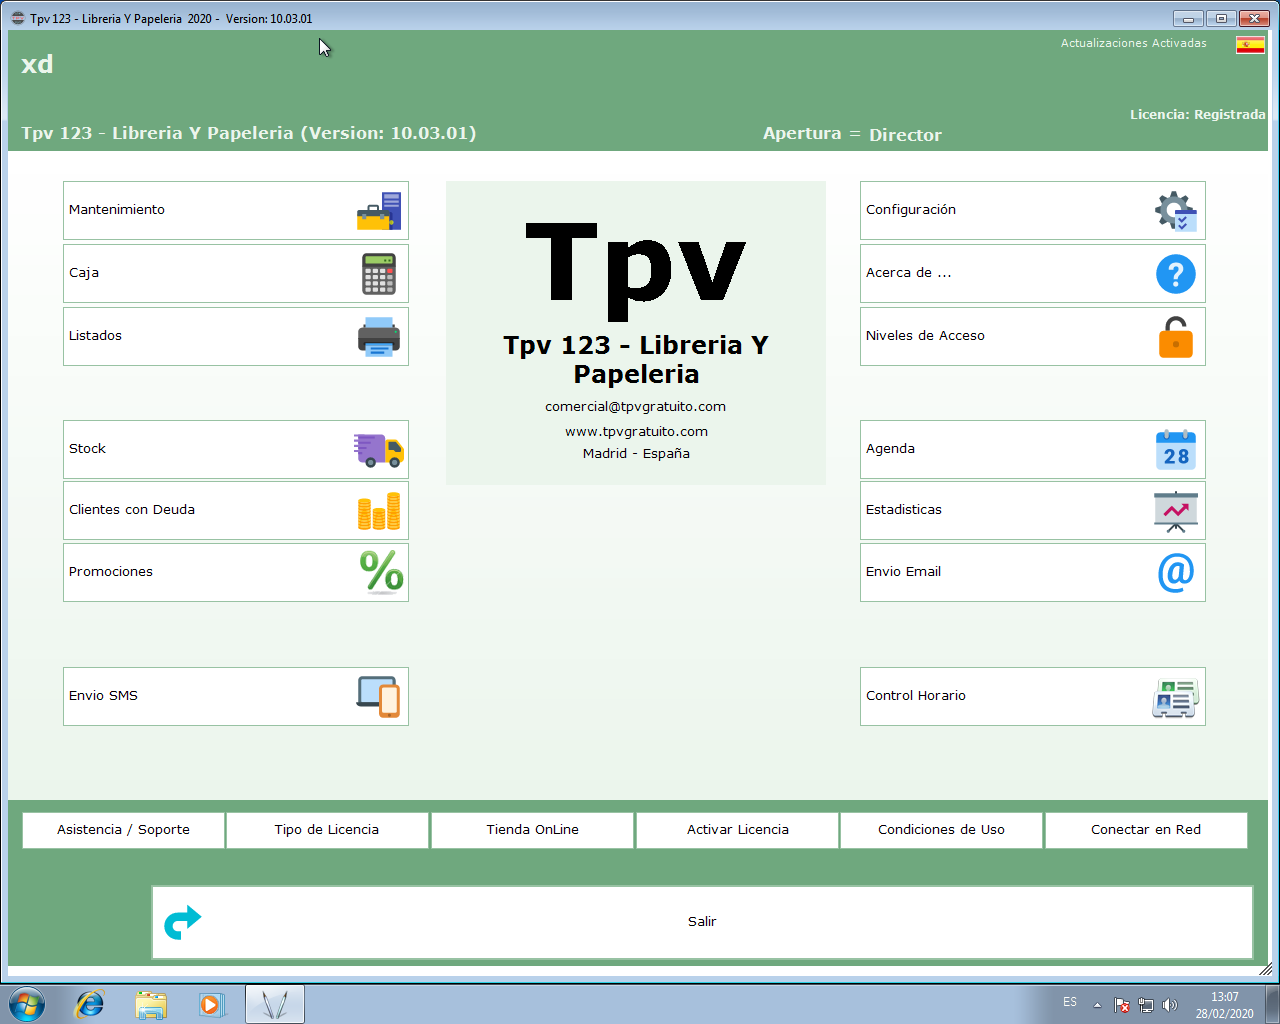
\includegraphics[scale=0.35]{tpv.png}
\end{figure}
\newpage
\section{Análisis del software: ISO 9001}
\subsection{Objetivo y campo de acción}
\paragraph{Este programa esta desarrollado para cubrir las principales necesidades de aquellas empresas que se dedican a la venta minorista de productos con código de barras o códigos propios}
\paragraph{este software fue desarrollado por SolverMedia SL. organización que la estableció e implementó la aplicación en el año 2008 y aun mantiene su sistema de gestión de la calidad y mejorando continuamente su eficacia.}

\subsection{Sistema de gestión de calidad}
\subsection*{Requisitos generales}
\paragraph{El producto se desarrolló con el fin de satisfacer las necesidades básicas de las PYMES la cual es mantener un control digital y seguro que se encarga de mantener una imagen fiel de la situación económica de la empresa, ademas de contabilizar el inventario existente en dicha entidad.}
\paragraph{Se desarrolló esta aplicación para que tuviera compatibilidad con el sistema operativo Windows en cualquier version vigente. Cuenta con una version libre con varias funcionalidades, sin embargo se puede comprar una licencia para apoyar a los desarrolladores.}
\paragraph{El software cuenta con un manual de usuario donde detalla los siguientes puntos:}
\subsubsection*{Como instalar el programa}
\subsubsection*{Condiciones de equipo.}
\paragraph{Especifica los requisitos mínimos que debe que tener el hardware y software del equipo en el que se va a instalar el programa para que funcione me manera optima}
\subsubsection*{Detalles de la interfaz principal.}
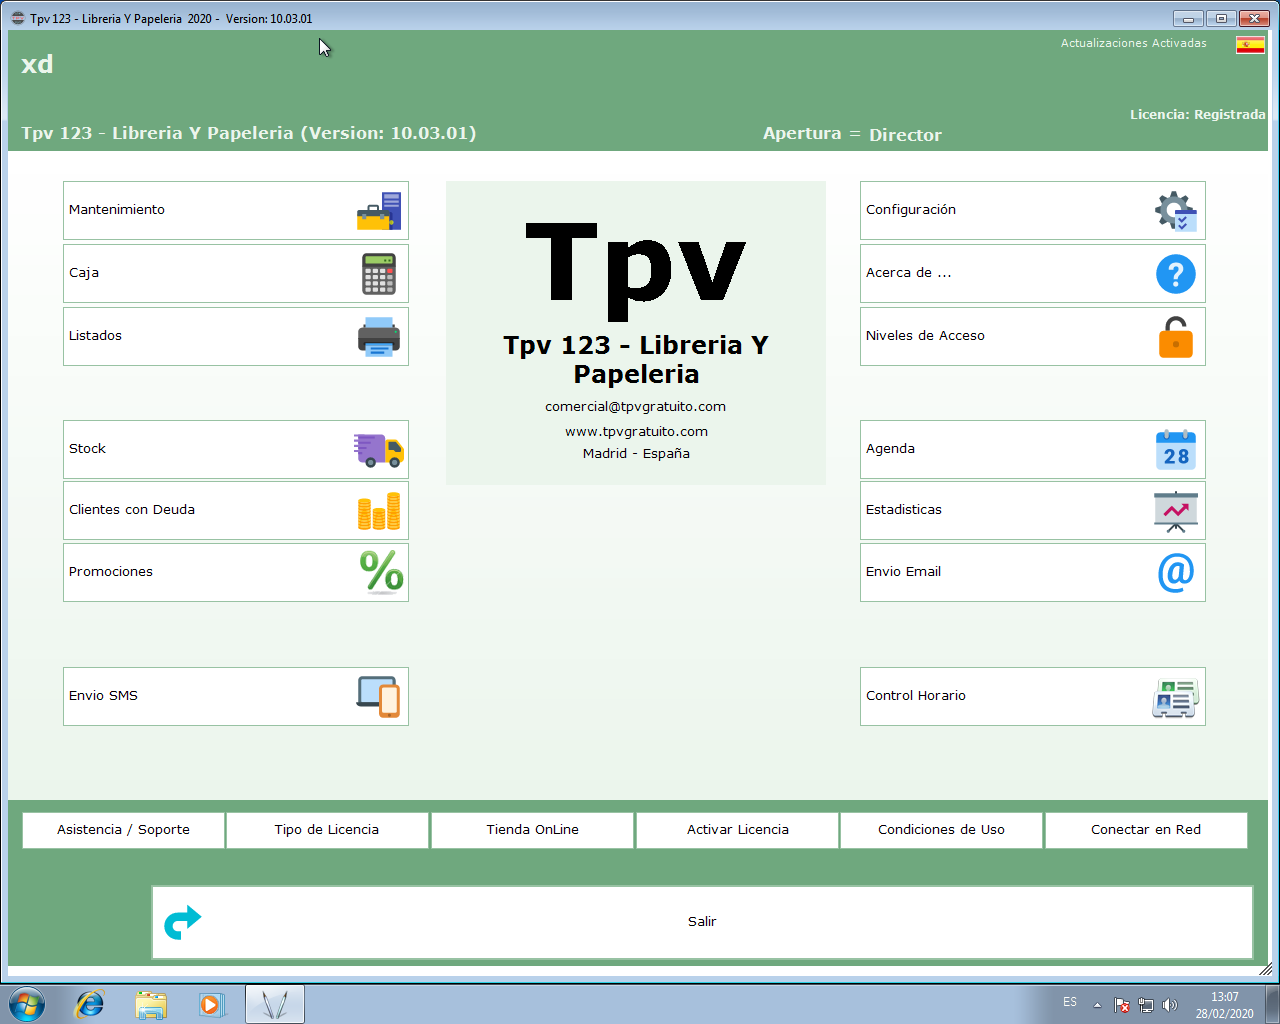
\includegraphics[scale=0.35]{tpv.png} 
\paragraph{Muestra la usuario el conjunto de funcionalidades principales con el que cuenta el sistema las cuales dan soluciones a las siguientes necesidades}

\subsubsection*{Configuraciones optimas para el sistema.}
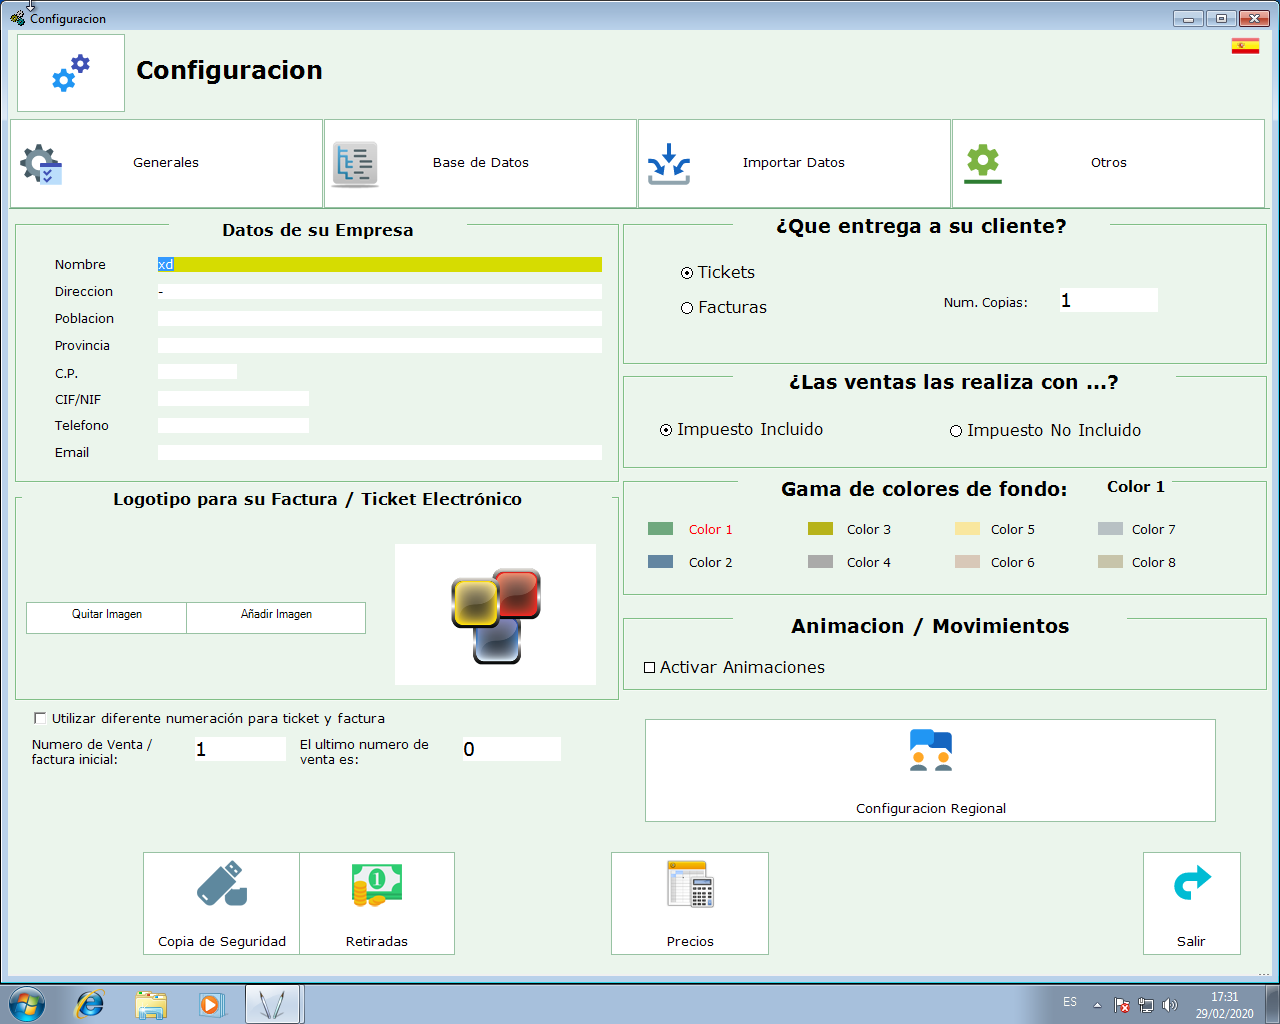
\includegraphics[scale=0.35]{Configuracion.png}
\paragraph{Esta sección le permite al usuario detallar los datos de su empresa, establecer el diseño de la factura, Realizar copias de seguridad automática para evitar perdida de datos, detalles de impuestos y los precios} 

\subsubsection*{Detalles de mantenimiento }
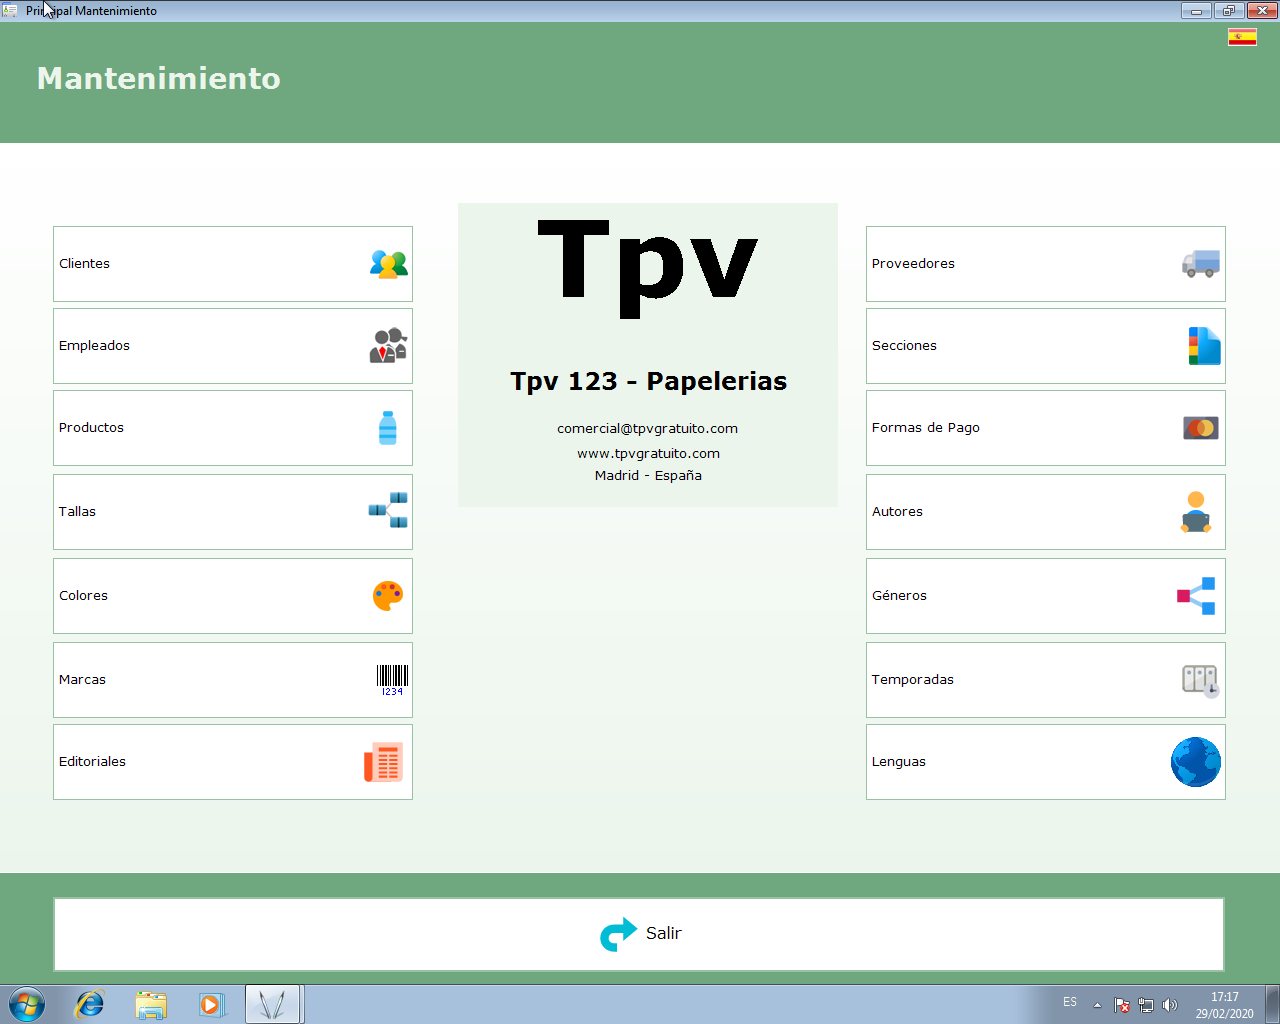
\includegraphics[scale=0.35]{Mantenimiento.png} 
\paragraph{Con esta sección el usuario podrá registrarse los productos, métodos de pagos, empleados,códigos de productos y los proveedores}

\subsubsection*{Funciones de caja}
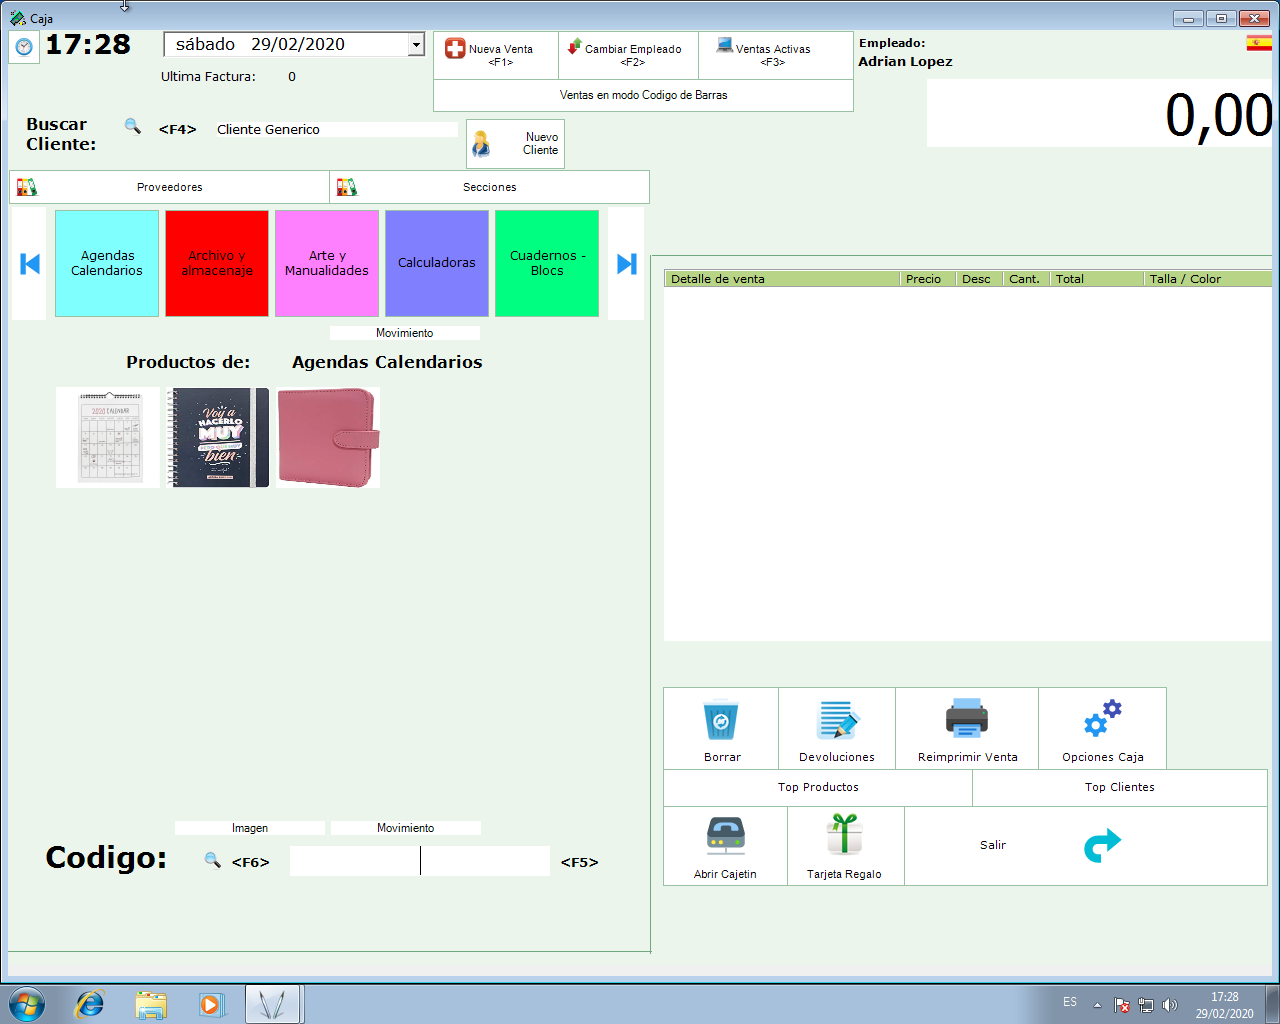
\includegraphics[scale=0.35]{Caja.png} 
\paragraph{Permite al encargado de la caja el poder seleccionar los productos ingresados con su respectivo código, precio y la cantidad para así poder generar una factura que será entregada al cliente}

\subsubsection*{Control de stock}
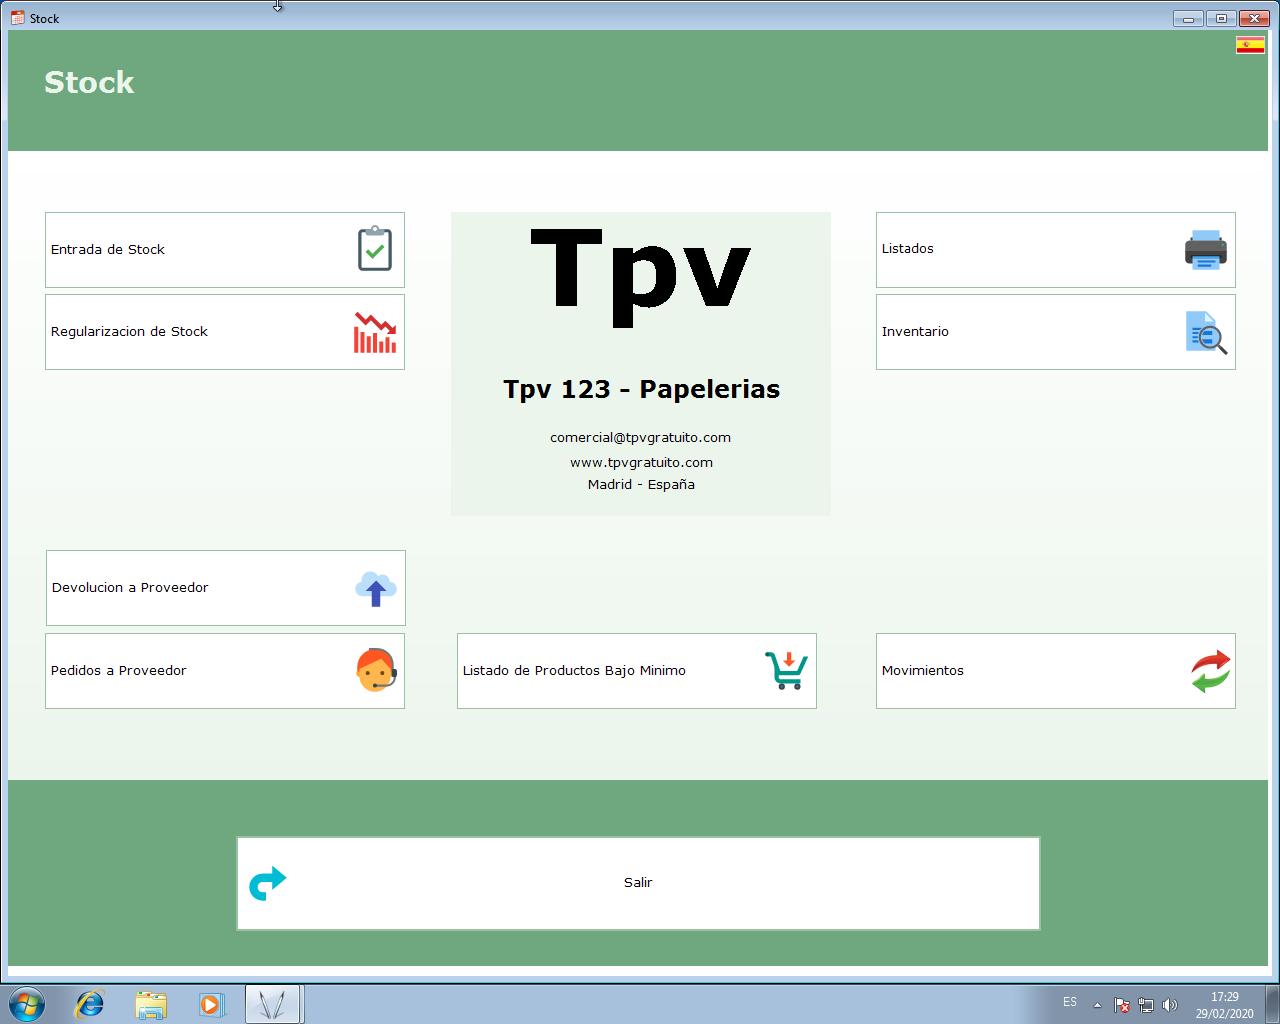
\includegraphics[scale=0.35]{Stock.png}
\paragraph{Permite visualizar al personal de trabajo la situacion del inventario (productos existentes)} 

\subsubsection*{Gestionar clientes con deudas}
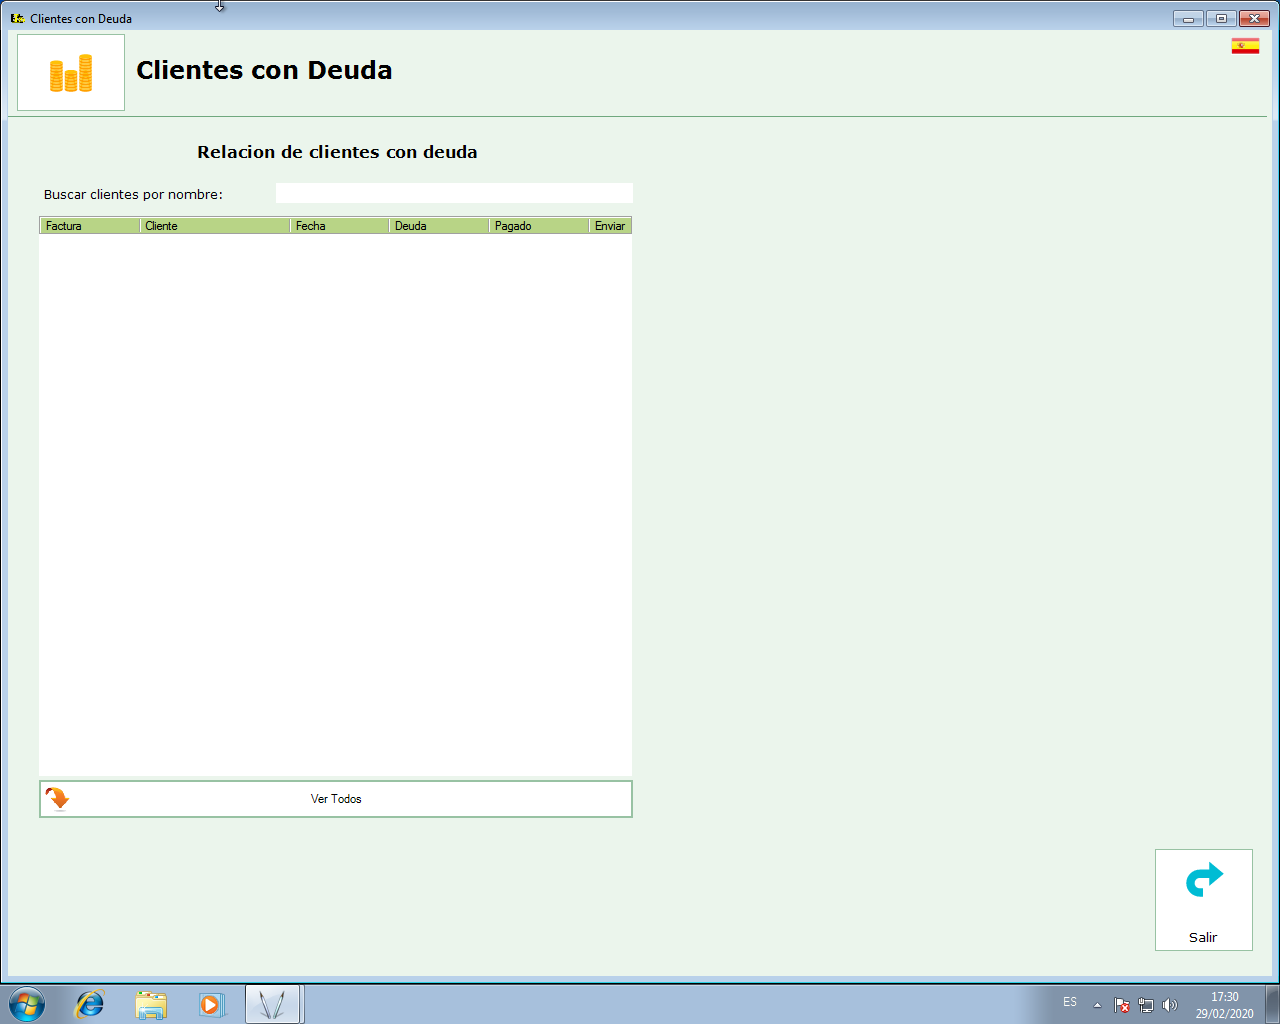
\includegraphics[scale=0.35]{Clientes con deuda.png} 
\paragraph{Mantiene el registro de aquellos clientes que mantienen una deuda con la entidad, muestra con detalles el monto pagado y el precio de deuda.}

\subsubsection*{Establecer promociones}
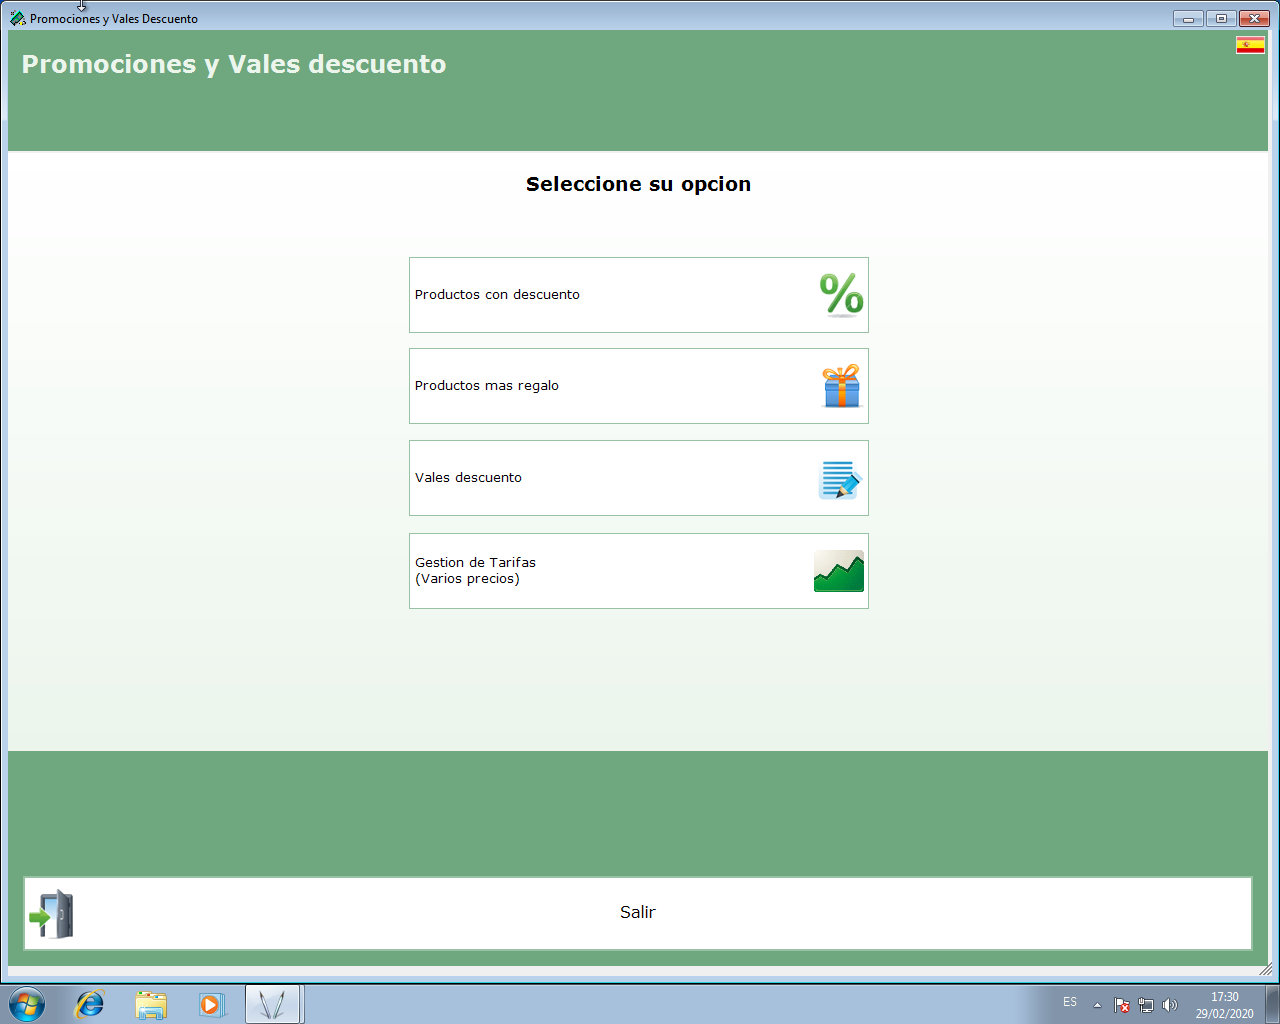
\includegraphics[scale=0.35]{Promociones.png} 
\paragraph{Permite ingresar o eliminar un producto por medio del código y establecer un porcentaje de descuento}

\subsubsection*{Configurar los niveles de acceso}
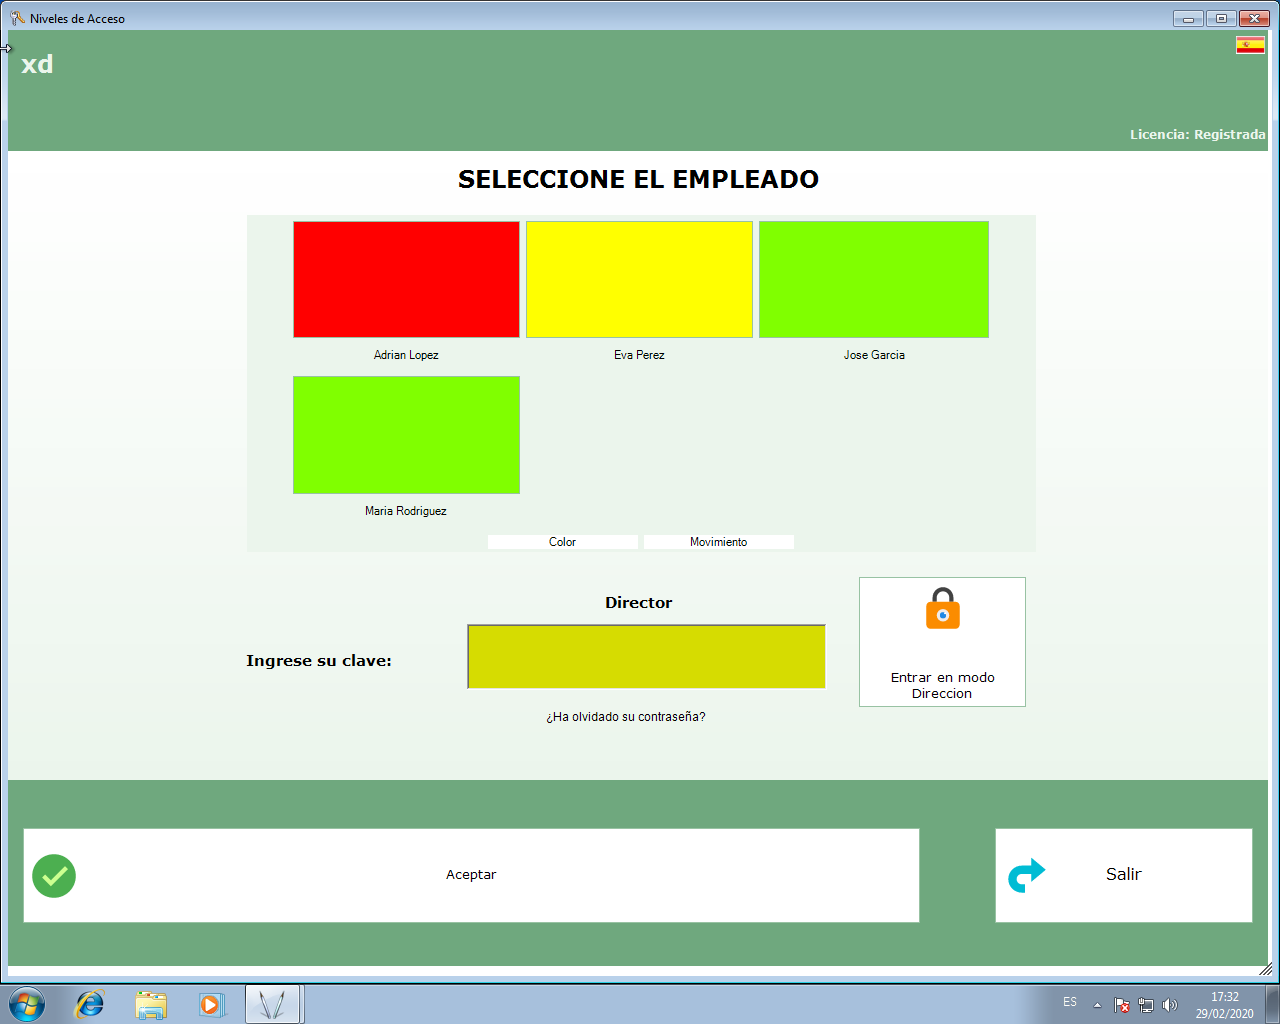
\includegraphics[scale=0.35]{Niveles de acceso.png}
\paragraph{Esta sección le permite al gerente de la empresa que va a adquirir el software controlar el acceso a la información para evitar que los datos sean alterados} 

\subsubsection*{Enviar mensajes}
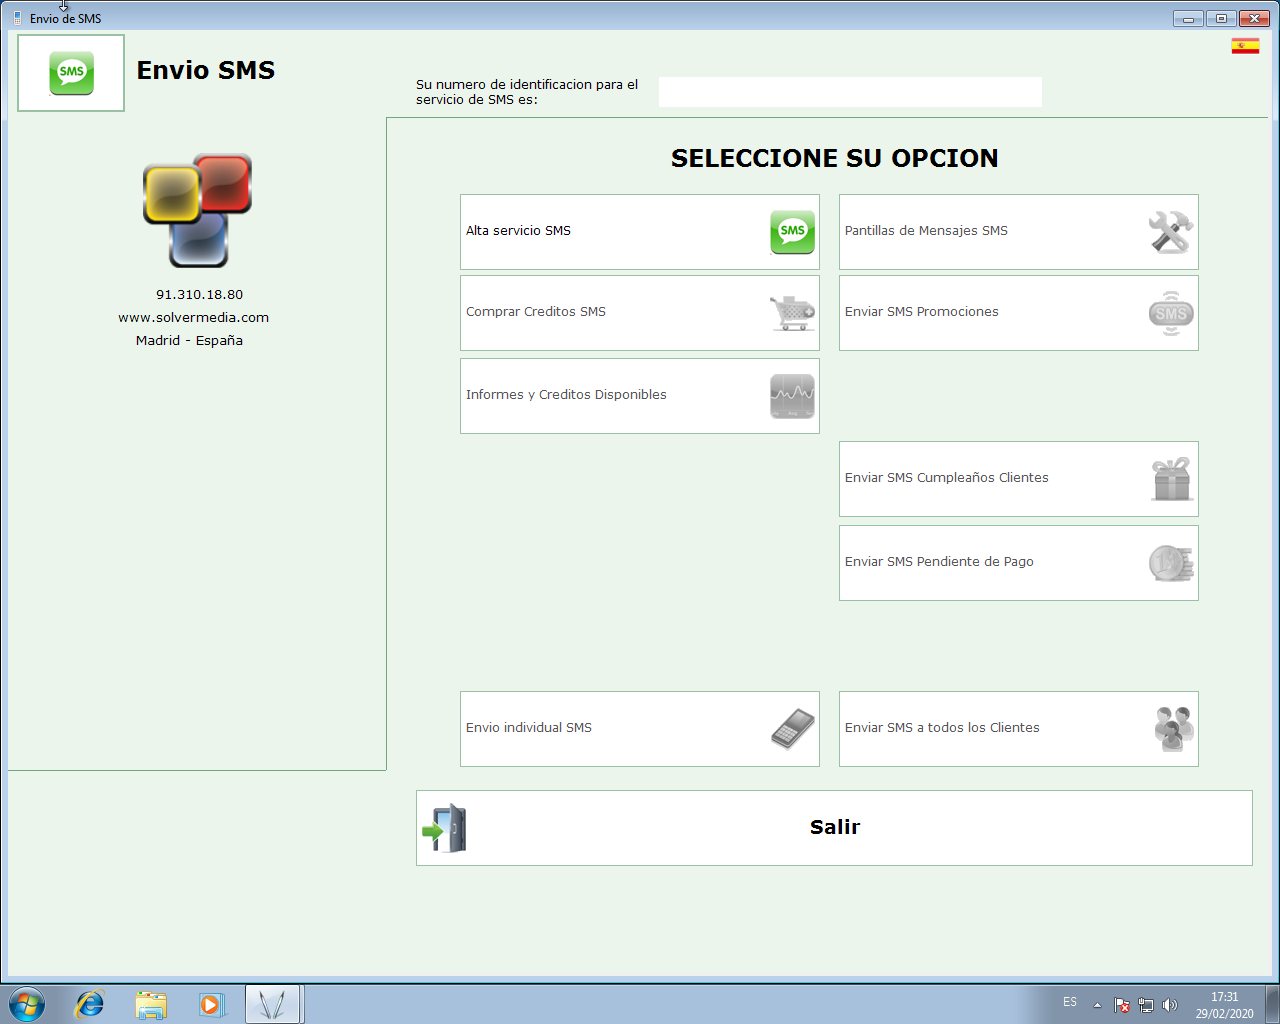
\includegraphics[scale=0.35]{Envio SMS.png}
\paragraph{Esta sección soluciona el problemas de comunicación entre sucursales en caso de que la entidad cuente con mas de un establecimiento} 

\subsubsection*{Condiciones de uso }
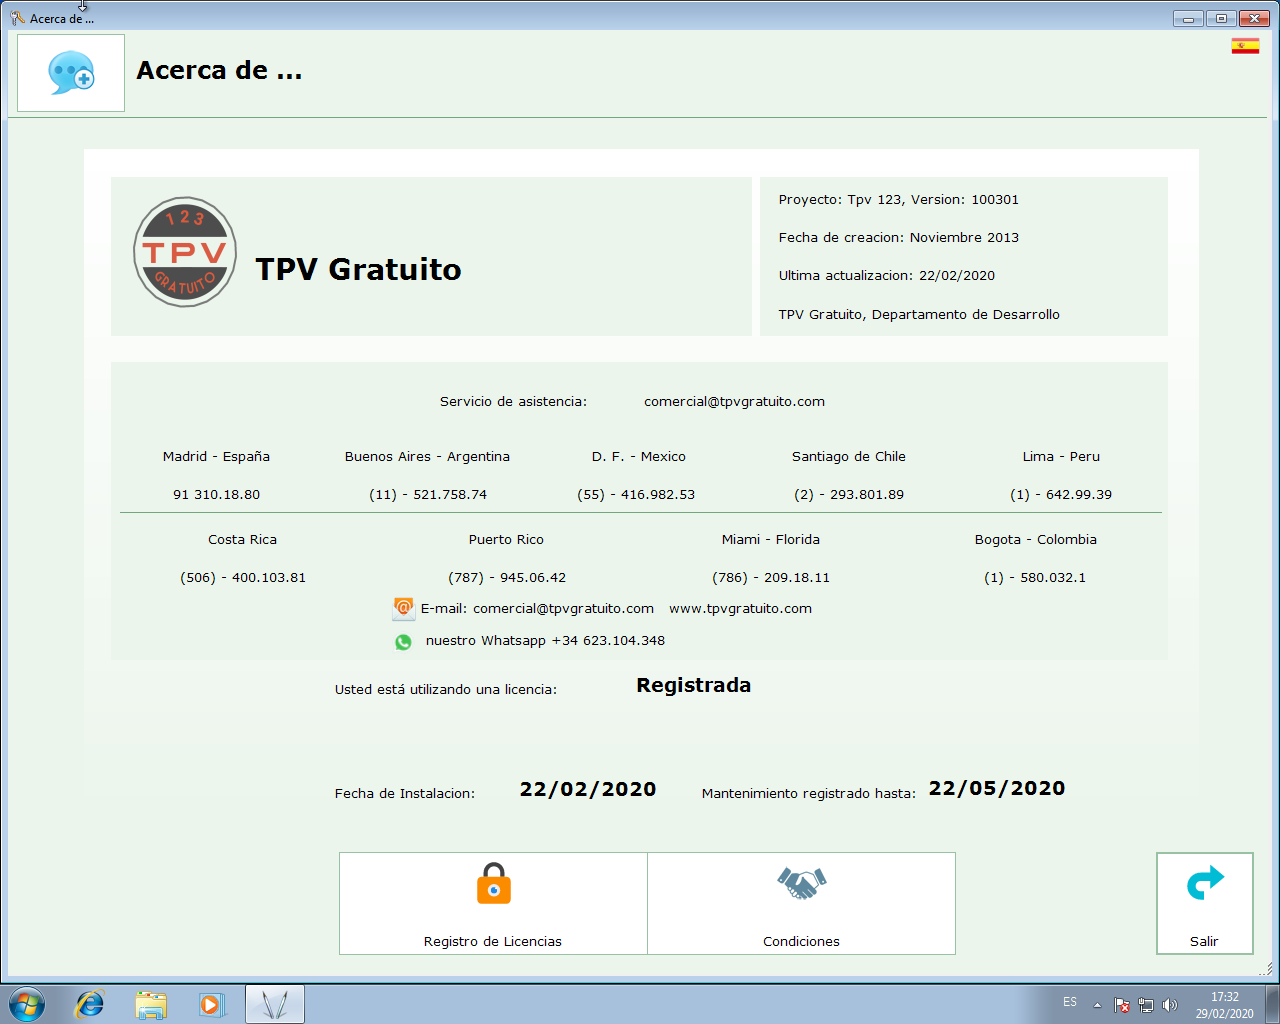
\includegraphics[scale=0.35]{Acerca de.png} 
\paragraph{Indica la responsabilidad que tiene el beneficiario con el software.}

\paragraph{Nota: No se encuentra existencia de un manual técnico que sea de dominio publico, solo queda suponer que si fue realizado.}
\paragraph{No se encuentran detalles del proceso de elaboración del software, ni el tipo de modelo de desarrollo que nos indique la evolución del sistema como tal.}
\paragraph{Aunque no se encuentra detalles de elaboración del software debido a que no es de código abierto se puede evidenciar la calidad del sistema ya que tiene una aceptación de 4.5/5 según la comunidad donde se encuentran comentarios positivos de personas que han utilizado este software, con ello se puede evidenciar la calidad del software que es el enfoque principal del estándar ISO 9001.}



\end{document}
